\chapter{SYSTÈMES DE GESTION HÔTELIÈRE}
\section{GESTION HÔTELIÈRE AU CAMEROUN}

Avec des besoins technologiques grandissants, les hôteliers font face à de nouveaux défis, dont celui d’investir dans des systèmes de gestion performants. C’est dans un souci de compétitivité que l’inter connectivité entre les différentes interfaces prend de l’importance, même si la tâche peut s’avérer ardue. La justification de tels investissements demeure néanmoins un perpétuel défi pour les gestionnaires\\

Bien que la plupart des établissements hôteliers dans le utilisent aujourd’hui des systèmes de gestion, ceux-ci sont presque tous dotés de fonctionnalités basiques comparativement à ce qui existe dans d’autres secteurs d’activité. Aujourd'hui, il existe de nouveaux outils appelés à devenir de véritables leviers de compétitivité des établissements hôteliers. On peut diviser les principaux systèmes de gestion en cinq catégories:
\begin{list}{•}{ }
\item base de données centrale: Property Management System (PMS);
\item réservations: Central Reservation System (CRS);
\item revenus: Revenue Management System (RMS);
\item points de vente: Electronic Point of Sale (EPOS);
\item Marketing: Customer Relationship Management (CRM)\\
\end{list}

Pour la gestion des opérations hôtelières, chaque département fonctionne avec un système différent. Le système PMS utilisé à la réception permet de gérer les activités quotidiennes (voir image ci-dessous), soit les arrivées et les départs des clients, la facturation, la gestion des chambres, etc. On s’en sert comme une centrale pour les systèmes des autres services afin de collecter toutes les informations des clients, notamment les factures du restaurant, des services aux chambres et des appels téléphoniques. Les systèmes PMS, CRS, RMS et CRM sont généralement connectés entre eux, ce qui permet de suivre les nouvelles réservations et de communiquer la disponibilité et les tarifs en temps réel.\\

On constate également un grand nombre d’hôtels de la place qui utilise encore des systèmes de gestion manuel. De la facturation a la gestion des réservations tout est fait manuellement et sur papier.\\

D’autre part les gestionnaires d’hôtel les plus averti ont eu vent des avantages du e-commerce et essaye de développer leurs activité grâce au service en ligne. Toute fois chaque hôtel possède son propre site qu’il présente individuellement à ses clients. Naviguer sur plusieurs sites web d’hôtel est extrêmement difficile et de la née le besoin de créer des plateformes qui ressemble un grand nombre d’hôtel ou les clients peuvent comparer les offres de chaque hôtel avant de s’engager dans une réservation. Hosteline se présente dans le registre des plateformes fédératrice d’hôtels tout comme booking.com et Jumia Travel qui vendent des produits qui appartient aux hôtels qui ont souscrit a leurs plateforme. On peut également lui donner la connotation de e-commerce dans le sens ou des clients achètent des produits et services par Hosteline.\\

Le plus difficile avec les plateformes ou on vend les produits des tierces personnes est de permettre au vendeur d’entretenir la relation client et de fidéliser sa clientèle. Ceci d’autant plus que la plateforme a des objectifs qui passent par la fidélisation des clients mais cette fois ci en vers le site de vente. Pour permettre aux hôteliers d’entretenir la relation client avec leurs clients sur la plateforme, Hosteline a pensé des stratégies parmi lesquels un système décisionnel qui servira les hôteliers et leurs clients mais Hosteline et ses clients. Cela permet de rapprocher le client et le vendeur et permettre une meilleure fourniture de service et une augmentation du chiffre d'affaire pour chacune des entreprises.\\


\section{PRÉSENTATION TECHNIQUE  DE HOSTELINE}
 Comme la majorité des projets informatiques, Hosteline a été conçu et réalisé selon un canevas avec des langages et méthodes de conception bien connu. En effet ce projet a été piloté par la méthodologie agile SCRUM (Annexe xx) avec le langage UML pour accompagne la conception. Après une description brève du langage UML, Les diagrammes qui ont servi à la conception de Hosteline seront présentés et commentés
 
 \subsection{LANGAGE UML}
 \textbf{UML} (Unified Modeling Language, que l’on peut traduire par langage de modélisation unifié) est une notation permettant de modéliser un problème de façon standard. Ce langage est né de la fusion de plusieurs méthodes existant auparavant, et est devenu désormais la référence en terme de modélisation objet, à un tel point que sa connaissance est souvent nécessaire pour obtenir un poste de développeur objet. La modélisation consiste à créer une représentation simplifiée d’un problème : le modèle. Grâce au modèle il est possible de représenter simplement un problème, un concept et le simuler. La modélisation comporte deux composantes :
 \begin{list}{•}{ }
 \item L’analyse, c’est-à-dire l’étude du problème
 \item La conception, soit la mise au point d’une solution au problème\\
 \end{list}

Le méta modèle UML fournit une panoplie d’outils permettant de représenter l’ensemble des éléments du monde objet (classes, objets, ...) ainsi que les liens qui les relie. Toutefois, étant donné qu’une seule représentation est trop subjective, UML fournit un moyen astucieux permettant de représenter diverses projections d’une même représentation grâce aux vues. Une vue est constituée d’un ou plusieurs diagrammes. On distingue deux types de vues :

i)	\textbf{Les vues statiques}, c’est-à-dire représentant le système physiquement
	\begin{list}{•}{ }
		\item diagrammes d’objets
		\item diagrammes de classes
		\item diagrammes de cas d’utilisation
		\item diagrammes de composants
		\item diagrammes de déploiement\\
	\end{list}
	 
ii)	\textbf{Les vues dynamiques}, montrant le fonctionnement du système
\begin{list}{•}{ }
		\item diagrammes de séquence
		\item diagrammes de collaboration
		\item diagrammes d’états-transitions
		\item diagrammes d’activités
	\end{list}

Mais en ce qui concerne notre cas d’étude présent, nous ne représenterons que les diagrammes utilisées lors de la conception de la plateforme Hosteline.

\subsection{DIAGRAMME DE CAS D’UTILISATION}

Les \textbf{diagrammes de cas d'utilisation} sont utilisés pour donner une vision globale du comportement fonctionnel d'un système logiciel. Ils sont utiles pour des présentations auprès de la direction ou des acteurs d'un projet, mais pour le développement, les cas d'utilisation sont plus appropriés. Un cas d'utilisation représente une unité discrète d'interaction entre un utilisateur (humain ou machine) et un système. Il est une unité significative de travail. Dans un diagramme de cas d'utilisation, les utilisateurs sont appelés acteurs (actors), ils interagissent avec les cas d'utilisation (use cases)[Source Wikipedia].

\begin{figure}[!htbp]
	\begin{center}
		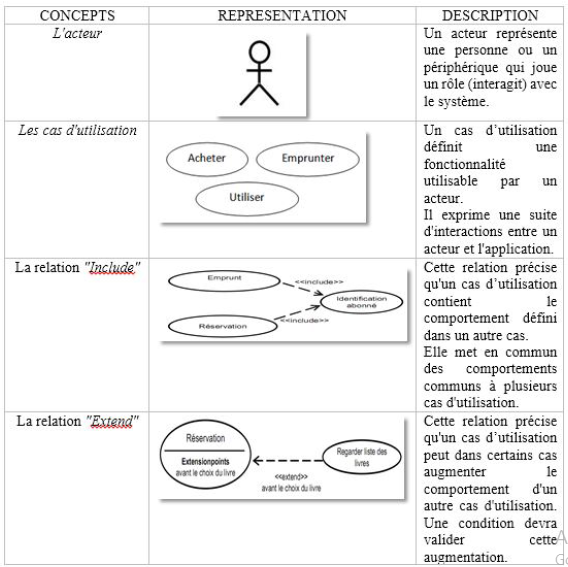
\includegraphics[scale=0.95]{images/form_use_case.png}
		\caption{Formalismes du diagramme de cas d'utilisation.}
		\label{use_case_summary}
	\end{center}
\end{figure}

\cleardoublepage

L’étude de Hosteline dans la partie diagramme de class à donner deux diagrammes représentent des groupes d’acteurs différents et ayant peu ou pas d’actions en commun comme le montrent les figures ci après.

\begin{figure}[!htbp]
	\begin{center}
		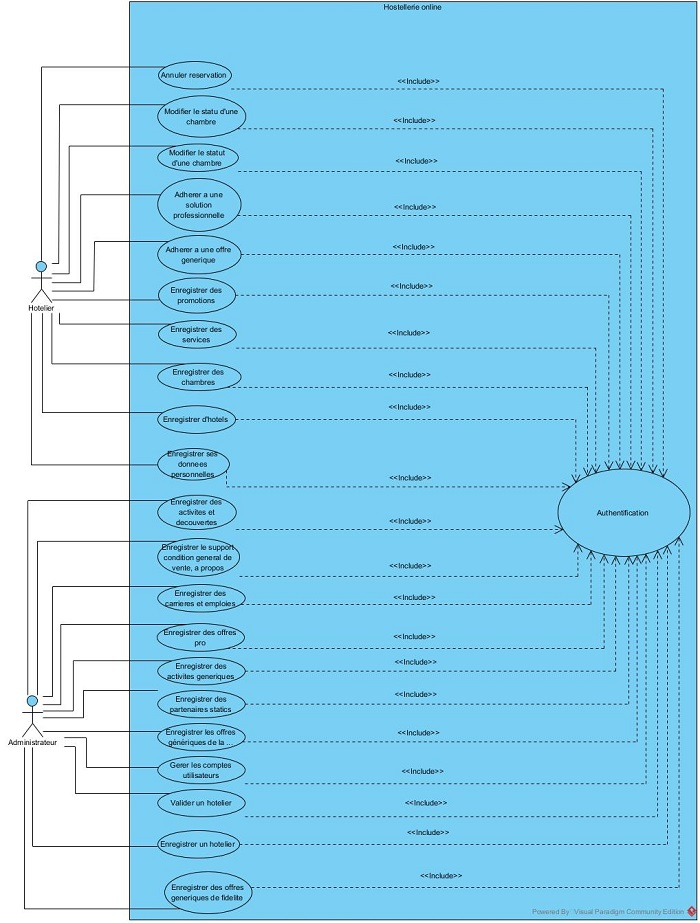
\includegraphics[scale=0.8]{images/diag_use_case2.jpg}
	\caption{Diagramme de cas d'utilisation contenant deux des acteurs de Hosteline (Agrandi en Annexe)}
		\label{use_case_diagramme_one}
	\end{center}
\end{figure}

\begin{figure}[!htbp]
	\begin{center}
		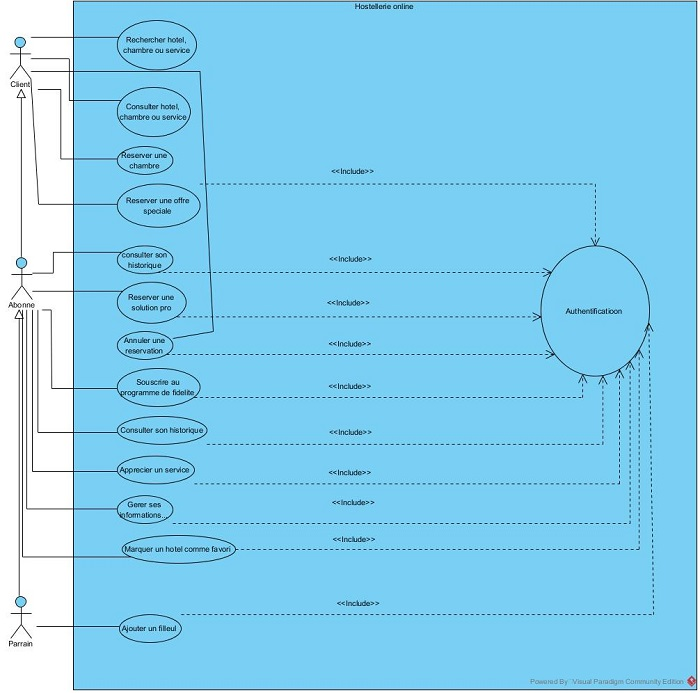
\includegraphics[scale=0.85]{images/diag_use_case1.jpg}
		\caption{Diagramme de cas d'utilisation contenant l'acteur "Client" (Agrandi en Annexe)}
		\label{use_case_diagramme_two}
	\end{center}
\end{figure}
\cleardoublepage
\subsection{DIAGRAMME DE CLASSES}

Le \textbf{diagramme de classes} est un schéma utilisé en génie logiciel pour présenter les classes et les interfaces des systèmes ainsi que les différentes relations entre celles-ci. Ce diagramme fait partie de la partie statique d'UML car il fait abstraction des aspects temporels et dynamiques.\\
Une classe est un ensemble de fonctions et de données (attributs) qui sont liées ensemble par un champ sémantique. Les classes sont utilisées dans la programmation orientée objet. Elles permettent de modéliser un programme et ainsi de découper une tâche complexe en plusieurs petits travaux simples.\\

\begin{figure}[!htbp]
	\begin{center}
		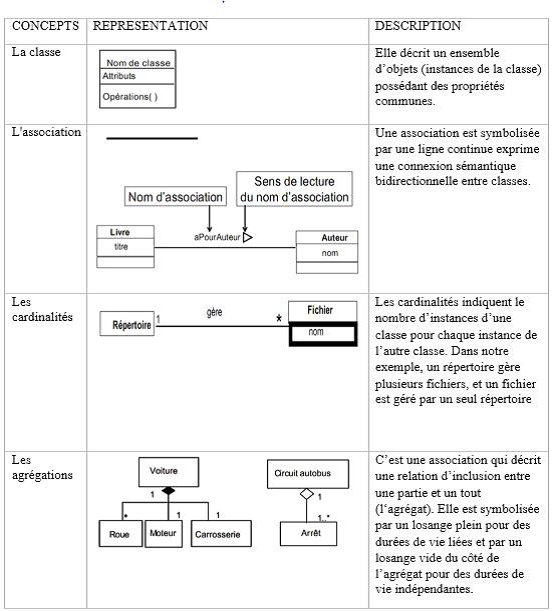
\includegraphics[scale=0.95]{images/form_classe.png}
		\caption{Formalismes du diagramme de classes.}
		\label{use_case_summary}
	\end{center}
\end{figure}
\cleardoublepage
En ce qui concerne Hosteline, dans sa phase d’étude le diagramme de classe qui en est sorti est celui de la figure suivante (Version agrandie en annexe).

\begin{figure}[!htbp]
	\begin{center}
		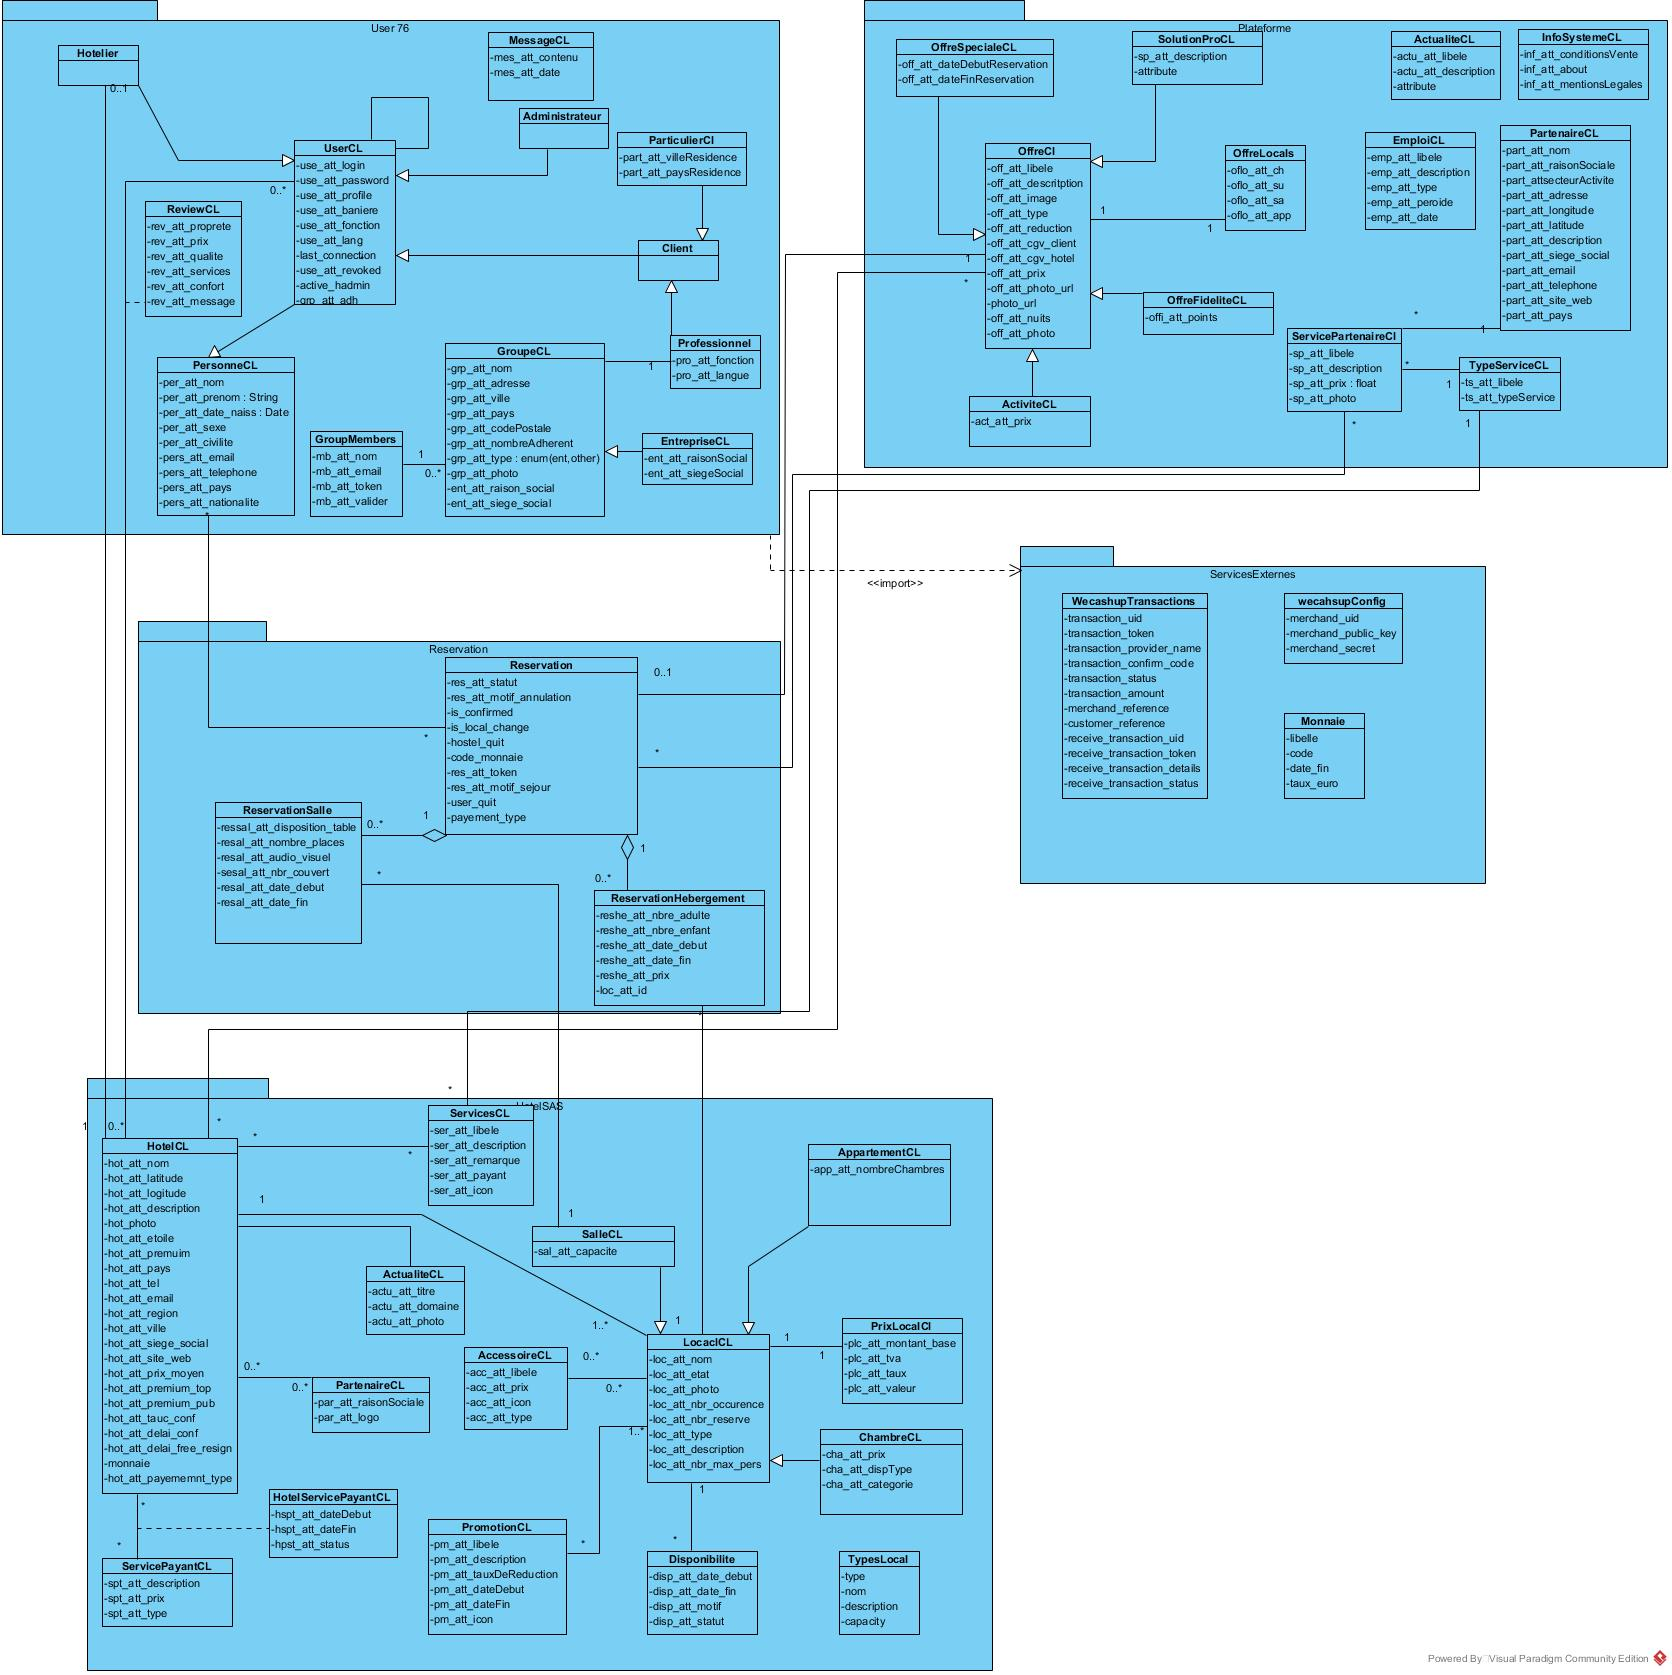
\includegraphics[scale=0.35]{images/diag_classe.jpg}
		\caption{Diagramme de classes du système (Agrandi en Annexe)}
		\label{classe_diagramme}
	\end{center}
\end{figure}
\cleardoublepage
\subsection{DIAGRAMME D'ENTITÉ ASSOCIATION}

Encore appelé diagramme d’entité relation (Entity Relation Diagram)

\begin{figure}[!htbp]
	\begin{center}
		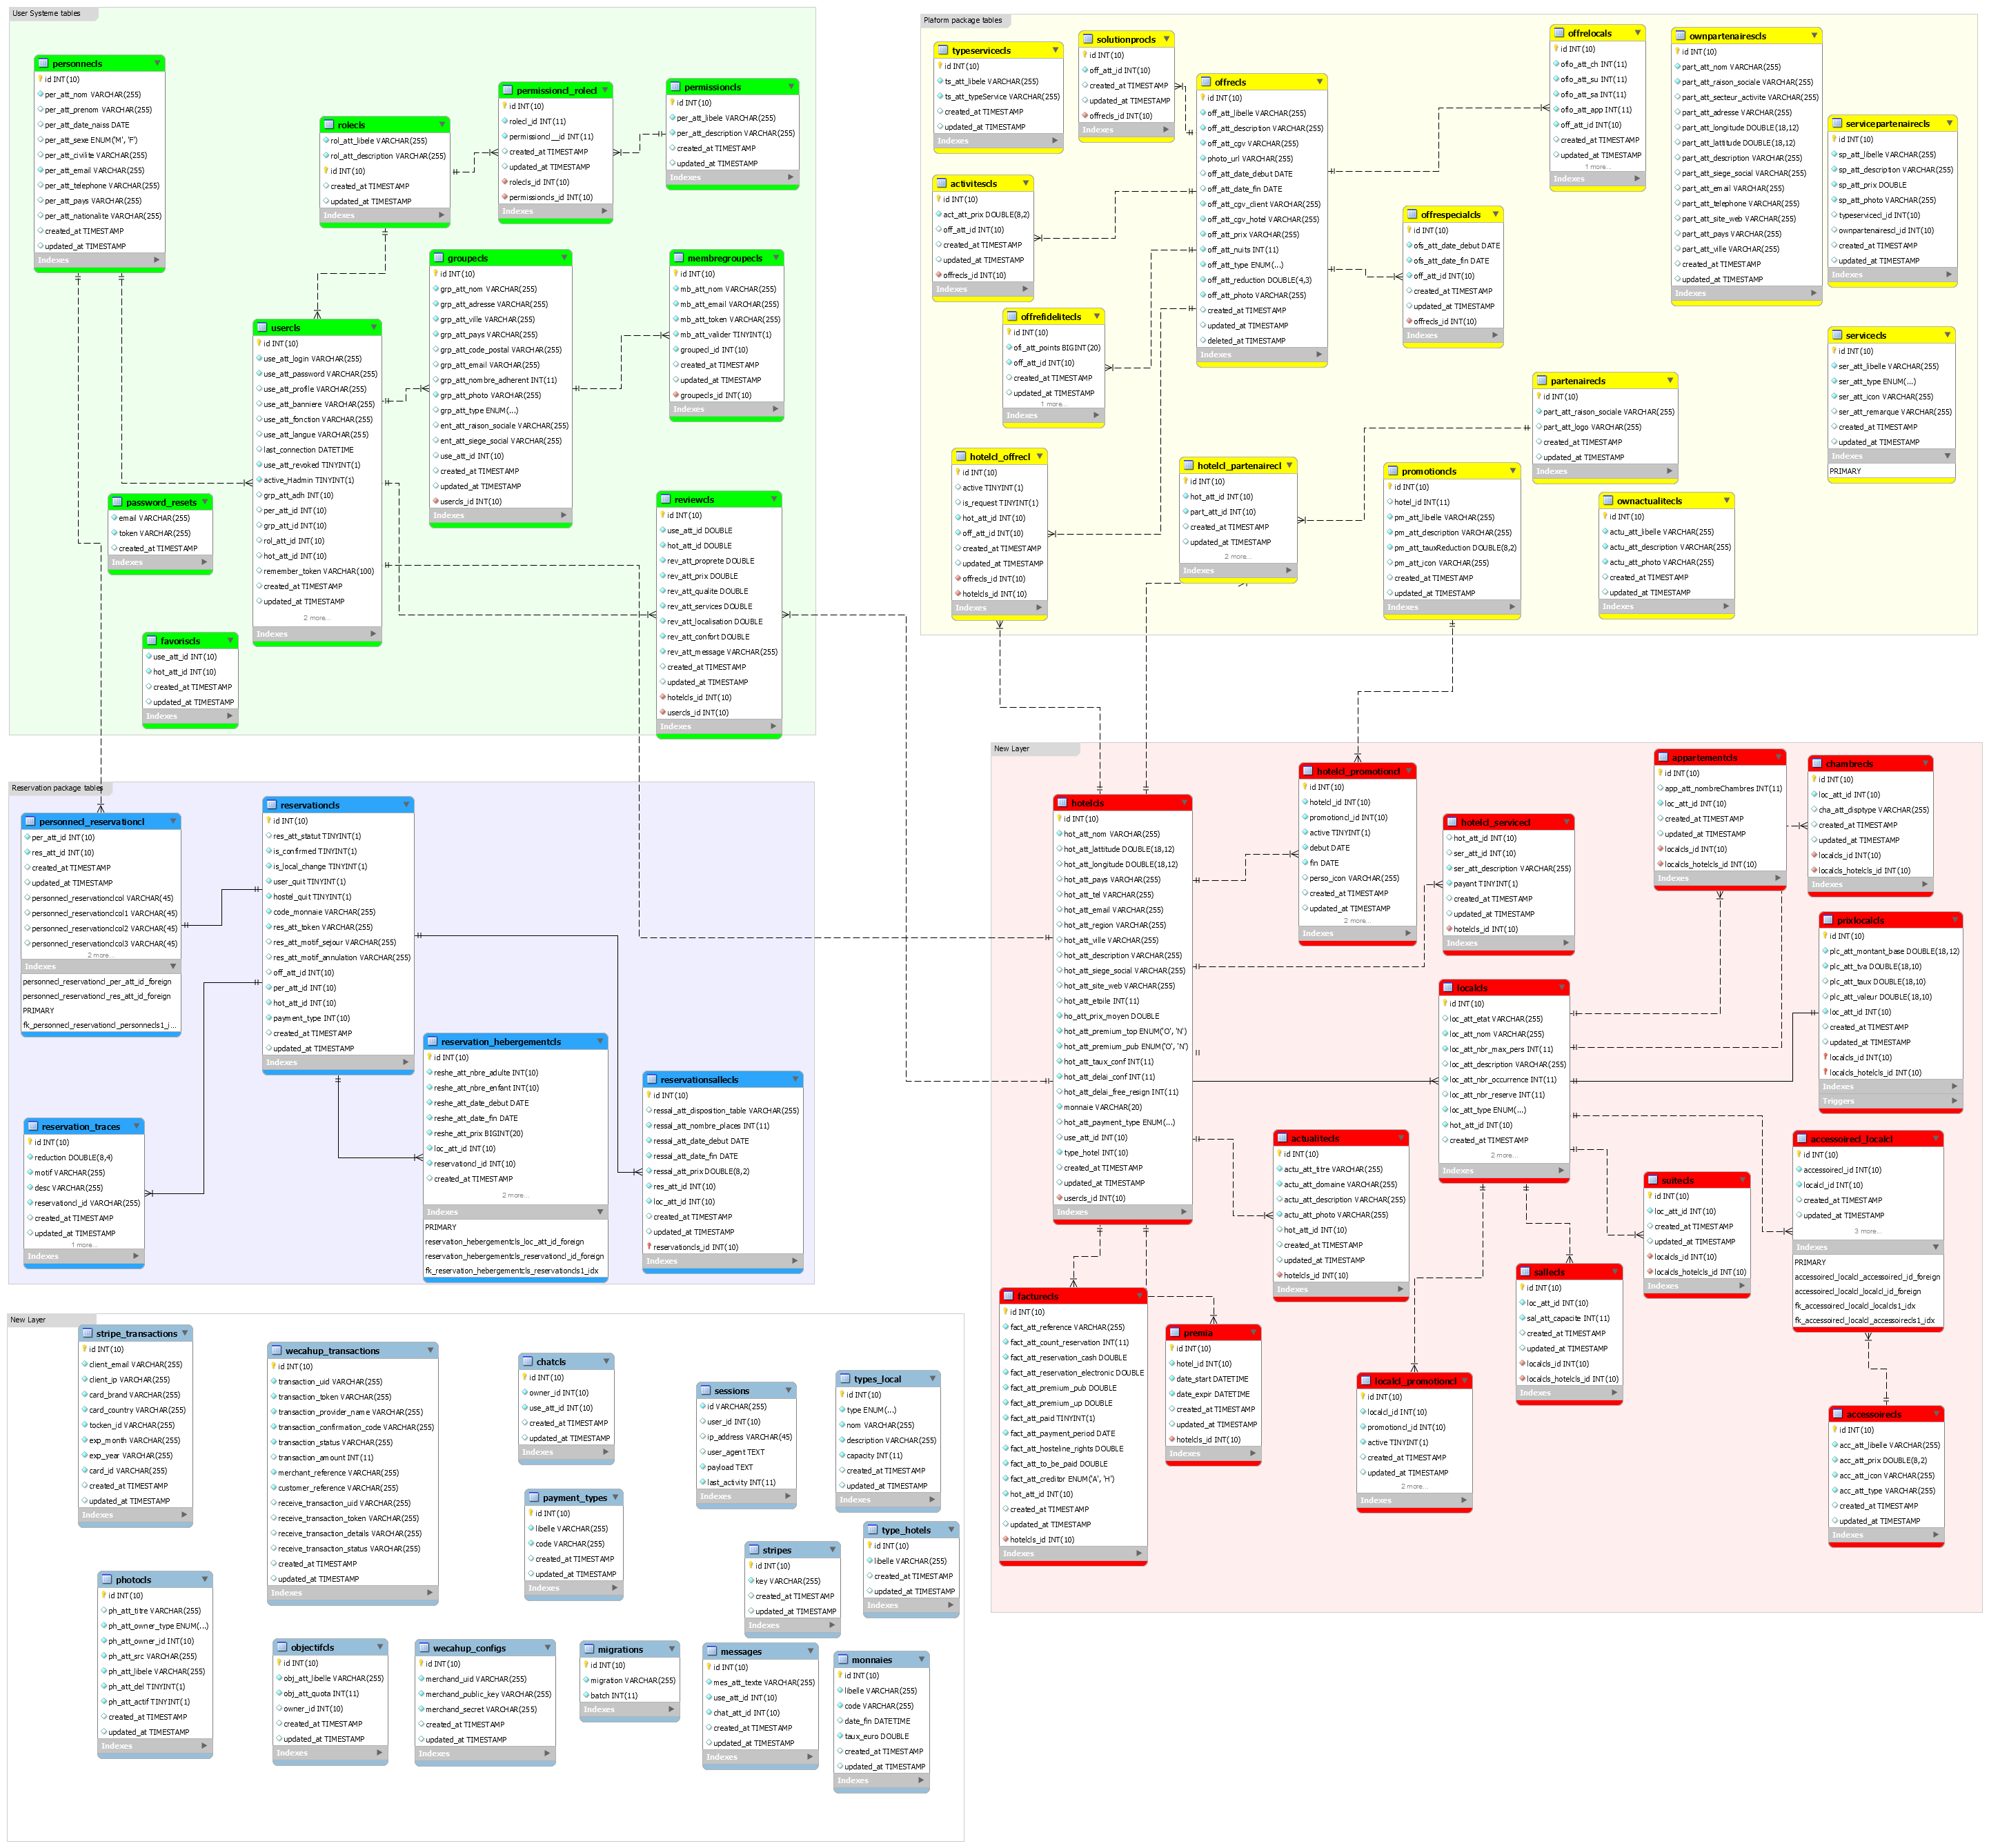
\includegraphics[scale=0.17]{images/diag_erd.png}
		\caption{ERD du système actuel (Agrandi en Annexe)}
		\label{classe_diagramme}
	\end{center}
\end{figure}

\cleardoublepage

\section{LE SYSTEME OPERATIONNEL ACTUEL}

Si on parle de mettre en œuvre un système décisionnel sur Hosteline c’est parce que un système opérationnel qui va fournir les données à ce dernier existe déjà et est tout à fait fonctionnel. Dans cette partie nous allons présenter des partie du Systèmes opérationnel par les quels la collecte de données est plus forte sur Hosteline.

\subsection{INSCRIPTION}	
L’inscription n’est pas une condition d’utilisation de Hosteline pour les clients qui souhaitent juste réserver. Elle est par contre le point d’entrée vers des droits et bonus supplémentaire pour le Client. Pour le Propriétaire d’hôtel ou client-hébergeur il doit s’inscrire pour avoir accès a l’administration de son établissement hôtelier. La figure en annexe XX montre comment se présente le formulaire d’inscription de Hosteline.

\begin{figure}[!htbp]
	\begin{center}
		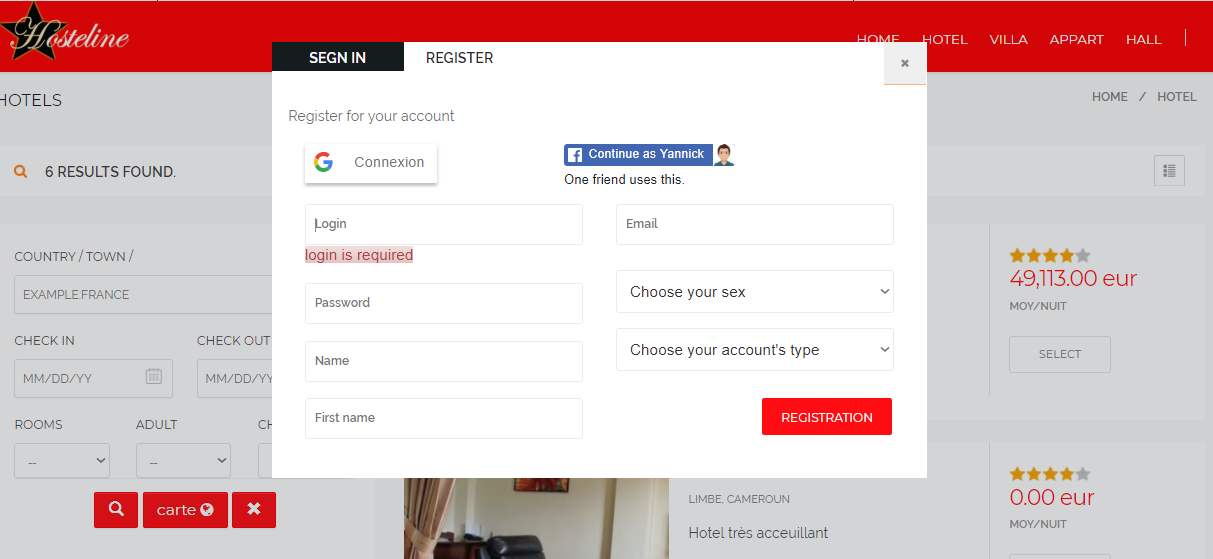
\includegraphics[scale=0.55]{images/inscription.png}
		\caption{ Interface d’inscription a Hosteline}
		\label{classe_diagramme}
	\end{center}
\end{figure}

\cleardoublepage
\subsection{LA RESERVATION}
La réserverions commence dès que l’utilisateur rentre ses critères de recherche car certain de ces critères seront retenu comme information de réservation. Le système de panier est utilisé ici et permet à l’utilisateur de sélectionner plusieurs chambres et de les réserver plus tard à sa guise. Lorsque la sélection est terminée l’utilisateur rentre ses informations s’il n’a pas de session en cours et valide sa réservation. Toute réservation validée peut être confirmé (Lorsqu’on paie) ou annulé suivant les termes et les conditions de l’hôtel et de la plateforme. La figure en Annexe XX est une capture de la fenêtre d’enregistrement des données de l’utilisateur.
\begin{figure}[!htbp]
	\begin{center}
		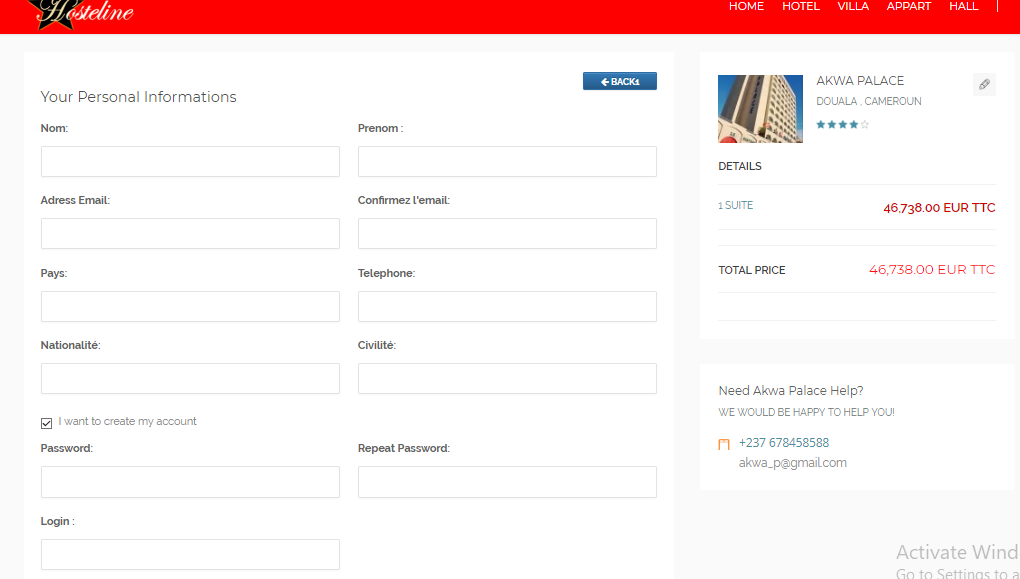
\includegraphics[scale=0.55]{images/reservation.png}
		\caption{Interface de réservations de Hosteline}
		\label{classe_diagramme}
	\end{center}
\end{figure}

\subsection{ENREGISTREMENT HOTELS}
Une fois le compte hôtelière crée, la prochaine étape consiste à créer son hôtel sur la plateforme et le configurer en y ajoutent des chambres, Sales et autre selon les dispositions de son établissement. En effet dans cette partie l’hôtelier ou la personne en charge du profile de l’hôtel va ajouter la description de son hôtel jusqu’à la position. La figure XX en annexe présente l’interface de création du profile d’un hôtel. 

\cleardoublepage
\section{LA PROBLÉMATIQUE DU THÈME}

INSBI propose des services à travers Hosteline sur un marché très concurrentiel car des plateformes comme celle-ci il y en a un grand nombre sur le marché. Pour gagner sa place et être concurrentiel, il y a lieux de développer des approches qui rendrons le produits plus intéressent que les autres déjà présent sur le marché. Dans un souci d’augmentation de la qualité des services offert aux clients, Les besoins suivants se sont formulés :
\begin{list}{•}{ }
\item\textbf{ Un tableau de bords pour chaque utilisateur :} Il s’agit de ressortir chaque profil d’utilisateur de la plateforme, revoir ses droit et ses actions sur la plateforme, et de déterminer les données génères par ce profile en suit de les traduire de manier graphique et interprétable. \\

\item\textbf{Pouvoir personnaliser les offres au client :} Le but étant de mettre sur pied un système permettant de mémoriser et restituer les choix des clients pour pouvoir leurs faire des offres a des périodes biens précises qui sont à la portée de leurs bourses. Le programme de fidélisation de Hosteline pouvant servir comme base pour le développement de ces outils. \\

\item\textbf{Etudie et faire de campagnes de publicité par localité :} Grace au donnée de localisation recueillit lors des réservations sur l’utilisateur et le lieu où il va passer les nuits on doit pouvoir faire une analyse croisé pour faire des promotions qui ciblent des clients d’un endroit précis ou des hôtels dans une location géographique précise.\\

\item\textbf{Veille environnementale :} Les outils développé a la suite du projet devront pouvoir intégrer des données de sources divers pour permettre d’informer les décideurs de l’évolution de l’environnement et des tendances qui tourne au tour du secteur hôtelier.\\
\end{list}

Après avoir écouté les besoins et les problèmes cité par les responsables de Hosteline nous avons entrepris une démarche projet pour résoudre méthodiquement les problèmes qui nous étaient posés et pour pouvoir aboutir à une solution qui répond a leurs besoins. Nous avons dans un premier temps nous référer aux diagrammes et modèles utilises a la conception de la plateforme pour avoir une idée claire de la structure des données en suit nous allons concevoir un data warehouse qui sera interrogé a l’aide d’un système de requêtes pour répondre aux questions des décideurs de la plateforme.\\

Dans le prochain paragraphe nous proposons de solutions et évaluons des choix d’outils pour implémenter ces solutions.

\cleardoublepage
\section{SOLUTIONS PROPOSÉES}

Parmi les solutions que nous avons développées pour INSBI, on pouvait dénombrer des solutions de reppoting, tableaux de bord et toutes ces solutions avaient un point en commun. Il fallait au départ construire un entrepôt de données et mettre sur pied un système d’exploitation de ces données qui permet de résoudre chaque problème à sa manière. Pour chaque problème nous avons fait des propositions de solutions et celle qui ont été retenues sont citée plus bas.

\begin{list}{•}{ }
\item Pour le \textbf{tableau de bords par profile utilisateur} nous avons proposé de développer un système décisionnel cote à cote au système opérationnel principale. Il s’agit de concevoir un data warehouse qui est chargé en temps réel a chaque insertion dans la BD opérationnel. Grace à cette solution la mise à jour des donnée du Data warehouse est instantanée (Entrepôt de données temps réel).  Ainsi les besoins explicites sont satisfaits grâce aux requêtes SQl spécialisés.\\

\item Pour permettre de \textbf{personnaliser les offres aux clients} nous avons assimilé ces problèmes à des problématiques connues et avons adopté des solutions connues que nous avons ensuite développé. Ici il ne s’agit de rien d’autre que le Data Minning (encore appelé Forage de données). Les données de chaque profil utilisateur sont traitées séparément et on peut extrapoler pour obtenir une tendance générale et proposer des offres qui vont satisfaire des profils groupé d’utilisateurs. Bien sûr ceci passe également par la mise sur pied d’un data warehouse spécialisé.

\item Face au besoin de \textbf{faire des offres localisé}, nous avons proposé de nous aider de donnée utilisateurs recueilli lors des réservations pour produire des représentations graphiques mettant en exergues les localités ou  les destinations et les taux de réservations correspondants. Grace aux chiffres représente par localité, les décideurs de Hosteline pourront a tout instant donné lancer des campagnes stratégiques qui leurs permet de faire un chiffre d’affaire plus grand.\\

\item Le problème de \textbf{veiller sur l'environnement} étais le plus difficile à résoudre car celui-ci fessait intervenir des données issues de l'environnement externe a Hosteline. Apres avoir identifié ces sources de données qui étaient de nature divers nous avons décidé d’exploiter des outils de BI spécialisés dans le traitement de données. Ici il fallait consolider les données internes et externes à Hosteline pour pourvoir en informations les décideurs de Hosteline. Pour mettre ça en œuvre le choix de l'outil \textbf{Pentaho Data Integration} a fait l'unanimité. Ici contrairement aux autres problèmes plus haut, la solution est totalement détachée de la plateforme web et sera déployé sur un serveur local a l’entreprise.

\end{list}


Les choix des techniques et technologies pour arriver aux solutions obtenues ont fait l’objet d’une étude préalable. Dans les chapitres suivants nous allons présenter les méthodes et les raisons qui nous ont permis de faire ces choix.

